\chapter{Predicting the Cross-Section}\label{ch:cross}

\begin{quote}\small\itshape
Before any model, understand the substrate. Cross-sectional return prediction
is not a hard instance of a standard machine-learning problem; it is a
different problem wearing the same clothes. This chapter fixes the task,
quantifies exactly how faint the signal is, and identifies the four features
of the environment --- noise, drift, dependence, and asymmetric error rewards
--- that dictate every design decision made in the rest of the book.
\end{quote}

\section{The object of study}\label{sec:object}

\subsection{Panels}

Everything in this book lives on a \emph{panel}: a set of entities (stocks)
observed jointly over time. Let $t = 1, \dots, T$ index trading dates and let
$\mathcal{U}_t$ denote the \emph{universe} at date $t$ --- the set of names we
are willing to trade and able to observe, with $N_t = |\mathcal{U}_t|$. The
universe changes over time as firms list, delist, merge, and enter or leave
an index; Chapter~13 is devoted to why getting $\mathcal{U}_t$ right (and not,
say, using today's universe throughout history) is a first-order correctness
issue rather than a detail.

For each name $i \in \mathcal{U}_t$ we observe features and, later, a
realized outcome:

\begin{definition}[The prediction task]\label{def:task}
At each date $t$, given features $\vx_{i,t}$ for every $i \in \mathcal{U}_t$,
produce scores $s_{i,t} \in \R$. The target is the \emph{forward return} over
a horizon of $h$ days,
\[
  y_{i,t} \;=\; \frac{P_{i,t+h} - P_{i,t}}{P_{i,t}},
\]
where $P_{i,t}$ is the (dividend- and split-adjusted) price. The task is
\emph{cross-sectional}: what is graded at date $t$ is the correspondence
between the ranking of $\{s_{i,t}\}_{i \in \mathcal{U}_t}$ and the ranking of
the realized $\{y_{i,t}\}_{i \in \mathcal{U}_t}$.
\end{definition}

Two structural remarks, both of which will matter enormously.

First, note what the task is \emph{not}. It is not forecasting the market:
whether stocks collectively rise or fall tomorrow contributes nothing to the
grade, because a constant added to every $y_{i,t}$ leaves all rankings
unchanged. The time-series problem (``will the index go up?'') and the
cross-sectional problem (``which names will outperform which?'') are
different problems with different difficulty profiles, and this book is about
the second. This is also an economic choice: a portfolio built to be long the
top-ranked names and short the bottom-ranked ones, in equal dollar amounts,
is approximately immune to the market's direction --- it monetizes exactly
the ranking skill being graded and nothing else. Chapter~16 makes this
construction precise (quantiles, turnover, costs); Chapter~13 goes further
and makes the \emph{target} itself market-neutral by residualizing returns
against a rolling market beta.

Second, the label spans time. The target $y_{i,t}$ is not knowable until date
$t+h$: a ``sample'' dated $t$ quietly reaches $h$ days into the future. This
banal observation has a sharp consequence --- any evaluation split that puts
date $t$ in the training set and any of $t+1, \dots, t+h$ in the test set has
\emph{leaked test-period prices into training labels}. The purging rule of
Chapter~15 (drop the last $h$ training dates before every test block) is
nothing more than this paragraph turned into an inequality, but the
prototype dissected in Chapter~\ref{ch:autopsy} is far from the only system
to have missed it.

\subsection{Two kinds of features}

The package splits features into two tensors, and the split is conceptual,
not cosmetic:

\begin{center}
\small
\begin{tabular}{@{}lll@{}}
\toprule
 & shape & meaning \\
\midrule
$\vx^{\text{seq}}_{i,t}$ & $(T_w, d_{\text{seq}})$ &
  a trailing \emph{window} of $T_w$ days of per-day channels \\
 & & (returns, ranged volatility, volume shocks, \dots) \\
$\vx^{\text{snap}}_{i,t}$ & $(d_{\text{snap}},)$ &
  a \emph{snapshot} of characteristics known at $t$ \\
 & & (momentum, size, short-horizon reversal, \dots) \\
\bottomrule
\end{tabular}
\end{center}

The sequence tensor exists to be summarized by a recurrent encoder into a
\emph{state}: ``what kind of market has name $i$ been living in lately?'' The
snapshot tensor carries the cross-sectional characteristics that actually
differentiate names on a date. Keeping them separate keeps a later question
crisp --- \emph{who gets to see what?} In the architecture of Part~III, the
encoder's summary drives the regime gate, while the experts read the
snapshot; whether the experts should \emph{also} see the encoder state is a
genuine design decision (Decision~A) with arguments on both sides, and it is
decided, documented, and made switchable rather than picked silently.

Every feature carries one non-negotiable invariant:

\begin{definition}[Point-in-time discipline]\label{def:pit}
A feature value $\vx_{i,t}$ may depend only on information available at or
before date $t$. The target $y_{i,t}$ is the \emph{only} forward-looking
quantity in the panel, and it never appears inside a feature tensor.
\end{definition}

Definition~\ref{def:pit} sounds too obvious to state. It is stated because
violating it is the single most common way quantitative research fails, the
violations are almost never obvious (a volatility estimate computed over a
centered window; a rank normalization fitted on the full history; a
``reserved column'' in a feature matrix that turns out to be the target), and
because the violation \emph{always improves the backtest} --- an asymmetry we
return to in Section~\ref{sec:hostile}. In the package this definition is not
prose: it is a test (\code{test\_no\_lookahead}) that shifts the raw price
history and asserts which features are and are not allowed to change.

\subsection{Notation}

\begin{center}
\small
\begin{tabular}{@{}ll@{}}
\toprule
$i$, $t$ & entity (stock) and date indices \\
$\mathcal{U}_t$, $N_t$ & universe at $t$ and its size \\
$h$ & label horizon in days \\
$y_{i,t}$ & forward return over $(t, t+h]$ \\
$\vx^{\text{seq}}_{i,t}, \vx^{\text{snap}}_{i,t}$ & sequence window and snapshot features \\
$s_{i,t}$ & model score for name $i$ at date $t$ \\
$K$ & number of regimes / experts \\
$S_t \in \{1,\dots,K\}$ & latent regime state \\
$\pi_k$, $r_k$ & prior and posterior (responsibility) regime weights \\
$\gauss(y;\mu,\sigma^2)$ & Gaussian density in $y$ \\
$\IC_t$, $\ICbar$, $\ICIR$ & per-date rank correlation and its aggregates \\
\bottomrule
\end{tabular}
\end{center}

\section{The scale of the signal}\label{sec:scale}

The defining fact of this problem --- the one from which capacity control,
evaluation protocol, and multiplicity discipline all follow --- is that the
predictable component of the cross-section is \emph{tiny}. This section
quantifies ``tiny.''

\subsection{The information coefficient}

\begin{definition}[Rank information coefficient]\label{def:ic}
Fix a date $t$ with $N$ scoreable names. Let $\rho^{(s)}_{i}$ and
$\rho^{(y)}_{i}$ be the within-date ranks of the scores and of the realized
targets. The (rank) information coefficient at $t$ is the Pearson correlation
of the rank vectors,
\[
  \IC_t \;=\;
  \frac{\sum_i (\rho^{(s)}_i - \bar\rho)(\rho^{(y)}_i - \bar\rho)}
       {\sqrt{\sum_i (\rho^{(s)}_i - \bar\rho)^2}\,
        \sqrt{\sum_i (\rho^{(y)}_i - \bar\rho)^2}},
  \qquad \bar\rho = \tfrac{N+1}{2},
\]
i.e.\ the Spearman correlation between scores and outcomes across the date's
cross-section.
\end{definition}

Ranks rather than raw values for two reasons: returns are heavy-tailed
(Chapter~\ref{ch:regimes}), so a Pearson correlation on raw returns can be
dominated by a single outlier; and the trading construction we ultimately
grade against (sort names, go long the top, short the bottom) only consumes
the ranking anyway.

What is a \emph{good} IC? For daily-horizon equity signals, a persistent mean
IC of $0.02$--$0.05$ is respectable professional work; $0.10$ would be
exceptional. It is worth internalizing what such numbers mean in terms of
explained variance. For a correlation $\rho$ between score and outcome, the
fraction of cross-sectional variance explained by the best linear predictor
is $R^2 = \rho^2$. Thus:

\begin{center}
\small
\begin{tabular}{@{}ccc@{}}
\toprule
mean IC & $R^2$ & share of outcome variance that is noise \\
\midrule
$0.02$ & $0.0004$ & $99.96\%$ \\
$0.05$ & $0.0025$ & $99.75\%$ \\
$0.10$ & $0.01$   & $99.00\%$ \\
\bottomrule
\end{tabular}
\end{center}

A model at the top of the realistic range explains \emph{one quarter of one
percent} of what it is asked to predict. Machine-learning intuitions imported
from vision or language --- where a model failing to explain $20\%$ of the
variance is considered weak --- are not merely unhelpful here; they are
actively misleading about model capacity, about evaluation, and about what an
impressive-looking result probably is (Section~\ref{sec:hostile}).

\subsection{The null distribution: skill-free ICs are large}

The second half of the calibration is how big ICs are when there is
\emph{no} skill at all.

\begin{proposition}[Null variance of the rank IC]\label{prop:nullic}
Let the score ranking be independent of the outcome ranking (zero skill),
with no ties. Then
\[
  \E[\IC_t] = 0, \qquad \Var(\IC_t) = \frac{1}{N-1}.
\]
\end{proposition}

\begin{proof}
Condition on the outcome ranks; by independence the score ranks are then a
uniformly random permutation $\Pi$ of $\{1,\dots,N\}$. Write the IC as
$\IC = \sum_i a_i b_{\Pi(i)}$ where
$a_i = (i - \bar\rho)/\sqrt{\sum_j (j-\bar\rho)^2}$ and likewise $b$; both
vectors are centered ($\sum a_i = 0$) and normalized ($\sum a_i^2 = 1$).
Unbiasedness is immediate: $\E[b_{\Pi(i)}] = \frac1N \sum_j b_j = 0$. For the
variance, using $\E[b_{\Pi(i)}^2] = \frac1N\sum_j b_j^2 = \frac1N$ and, for
$i \ne i'$, $\E[b_{\Pi(i)} b_{\Pi(i')}] = \frac{1}{N(N-1)}\sum_{j \ne j'} b_j
b_{j'} = \frac{0 - \sum_j b_j^2}{N(N-1)} = -\frac{1}{N(N-1)}$:
\[
  \Var(\IC)
  = \sum_i a_i^2 \,\E[b_{\Pi(i)}^2]
  + \sum_{i \ne i'} a_i a_{i'} \,\E[b_{\Pi(i)} b_{\Pi(i')}]
  = \frac1N \;-\; \Bigl(\underbrace{\textstyle\sum_{i\neq i'} a_i a_{i'}}_{=\,0 - 1}\Bigr)\frac{1}{N(N-1)}
  = \frac1N + \frac{1}{N(N-1)} = \frac{1}{N-1}. \qedhere
\]
\end{proof}

So with $N = 100$ names per date, a \emph{zero-skill} model produces daily
ICs with standard deviation $1/\sqrt{99} \approx 0.10$ --- twice the size of
a genuinely good signal's mean. Figure~\ref{fig:nullic} shows the simulated
null: on roughly a third of all dates, pure noise scores $|\IC_t| > 0.10$.
Single-date (and single-month) performance is close to meaningless, and any
evaluation must aggregate.

\begin{figure}[t]
\centering
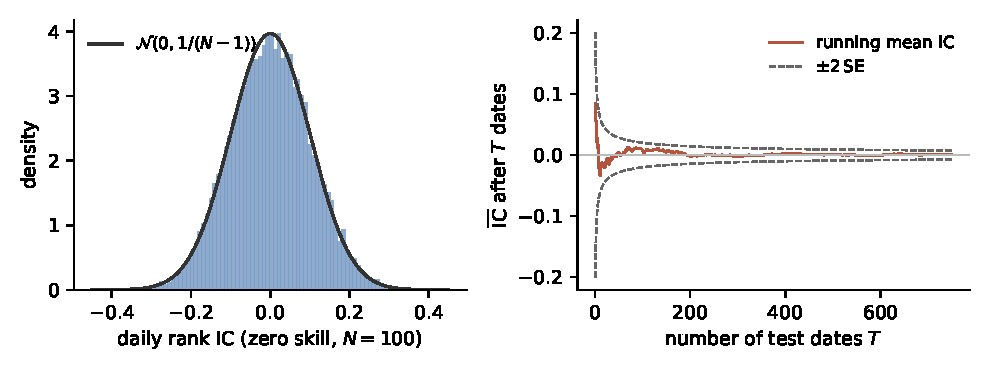
\includegraphics[width=\textwidth]{figures/null_ic.pdf}
\caption{\textbf{Zero skill produces large ICs.} Left: the simulated
distribution of the daily rank IC for a signal with no predictive content
($N=100$ names), with the $\gauss(0, 1/(N-1))$ overlay of
Proposition~\ref{prop:nullic}. Right: the running mean IC of one zero-skill
strategy over 750 test dates, against $\pm 2$ standard-error bands. Early
stretches of apparent skill (or anti-skill) of $|\ICbar| \approx 0.03$ ---
the size of a genuinely good signal --- are routine and mean nothing.}
\label{fig:nullic}
\end{figure}

\subsection{Aggregation and the arithmetic of proof}\label{sec:aggregation}

Average the daily series: $\ICbar = \frac1T \sum_t \IC_t$. If the daily ICs
were independent with standard deviation $\sigma_{\IC}$, the standard error
of the mean would be $\sigma_{\IC}/\sqrt{T}$, giving the $t$-statistic
\[
  t \;=\; \frac{\ICbar}{\sigma_{\IC}/\sqrt{T}}
    \;=\; \underbrace{\frac{\ICbar}{\sigma_{\IC}}}_{\textstyle\ICIR}
          \cdot \sqrt{T},
\]
where the ratio $\ICIR$ --- the per-date information ratio of the IC series
--- measures the signal's \emph{consistency}. This immediately yields the
book's first piece of experimental arithmetic: the number of test dates
needed before a true mean IC is statistically distinguishable from zero at
level $t^\ast$ is
\[
  T \;\geq\; \left( \frac{t^\ast \, \sigma_{\IC}}{\ICbar} \right)^{\!2}.
\]

\begin{example}\label{ex:arith}
A true $\ICbar = 0.03$ with realistic daily dispersion
$\sigma_{\IC} = 0.15$ (the null's $0.10$ plus regime-driven variation) needs
$T \ge (2 \times 0.15/0.03)^2 = 100$ test dates for $t = 2$, and $225$ dates
for $t = 3$ --- roughly five and eleven months of daily evaluation
respectively, \emph{if the daily ICs were independent}. They are not: with an
$h$-day label, adjacent dates share $h-1$ days of the outcome window, which
positively correlates the IC series and \emph{reduces} the effective $T$.
Every ``significant'' claim in this project is built to survive this
arithmetic; most published claims in the field would not.
\end{example}

\begin{engineering}[the evaluation harness]
This arithmetic is why the package's walk-forward harness
(\code{nec\_moe/evaluation.py}) pools ICs \emph{across all test dates of all
folds} before summarizing, reports $\ICbar$, $\sigma_{\IC}$, $\ICIR$ and
$t = \ICIR\sqrt{T}$ together rather than any of them alone, and why the label
overlap of Example~\ref{ex:arith} resurfaces twice: as the purging rule
(train/test separation must respect the $h$-day label span) and as a caution
against taking the nominal $t$-statistic at face value when $h > 1$.
\end{engineering}

\section{Why the problem resists standard machine learning}\label{sec:hostile}

Four properties of this environment, in increasing order of subtlety. They
are worth naming precisely, because each one dictates a specific piece of the
system built in this book.

\subsection{Noise dominates: variance is the binding constraint}

With $R^2$ of order $10^{-3}$, the mean-squared-error decomposition
\[
  \E\bigl[(\hat f(\vx) - f(\vx))^2\bigr]
  \;=\; \underbrace{\text{bias}^2}_{\text{model too simple}}
  \;+\; \underbrace{\text{variance}}_{\text{model too responsive to noise}}
\]
is wildly lopsided: the function $f$ being estimated is minuscule, while the
noise available for a flexible model to memorize is everything else. A model
class with the capacity to represent rich structure will, on a finite panel,
mostly represent noise. Concretely: a panel of $N = 500$ names over ten years
($T \approx 2{,}500$) has $1.25$ million rows, which sounds like plenty ---
until Section~\ref{sec:dependence} shreds the ``independent samples''
reading, and until one compares it with the four \emph{million} parameters of
the prototype's LSTM stack (Chapter~\ref{ch:autopsy}, defect~5). The
project's response is threefold: small encoders (a one-layer GRU with hidden
size 32, not an eight-layer LSTM), a mixture architecture whose components
are individually simple, and capacity-\emph{matched} baselines (Chapter~16)
so that any claimed advantage of the mixture cannot be an artifact of
parameter count.

\subsection{Nothing is stationary}

The mapping $\vx \mapsto y$ is not fixed. It drifts on two timescales.
Slowly: signals decay as they become known and traded away --- the
out-of-sample deterioration of published anomalies is one of the most robust
findings in empirical asset pricing (McLean and Pontiff, 2016, document
returns falling by roughly a third to a half after publication). And quickly:
the \emph{same} characteristic can predict with opposite signs in different
market states --- momentum's behavior in calm markets versus its crashes in
volatile rebounds being the canonical example, developed in detail in
Chapter~\ref{ch:regimes}. Slow drift motivates walk-forward evaluation
(train strictly on the past, test strictly on the future, refit as time
advances --- Chapter~15). Fast, recurring, state-dependent change is the
thesis itself: it motivates \emph{regime-conditional} models, in which the
cross-sectional mapping is allowed to depend on a latent market state. That
motivation is the subject of the next chapter, so here we only flag the
distinction: walk-forward handles drift you cannot model; regimes are a bet
that part of the drift is \emph{recurring structure} you can.

\subsection{Samples are deeply dependent}\label{sec:dependence}

The $1.25$ million rows above are not $1.25$ million observations in any
statistically meaningful sense.

\emph{Cross-sectionally}, names co-move through common factors: on a given
date, a large share of every stock's return is the market and industry
component. The effective number of independent observations per date is far
smaller than $N$. A back-of-envelope: if pairwise return correlations average
$\bar\rho_c$, the variance of the equal-weighted mean of $N$ names is
$\frac{\sigma^2}{N}\bigl(1 + (N-1)\bar\rho_c\bigr)$, so the effective sample
size is $N_{\text{eff}} = N / \bigl(1 + (N-1)\bar\rho_c\bigr)$; with
$\bar\rho_c = 0.25$ and $N = 500$, $N_{\text{eff}} \approx 4$ --- for
estimating the common component. Cross-sectional \emph{ranking} signals fare
better (the common component cancels between long and short legs, which is
precisely why the task is defined cross-sectionally), but the lesson stands:
row counts overstate information content by orders of magnitude.

\emph{Temporally}, overlapping $h$-day labels make adjacent dates share
outcome information (Example~\ref{ex:arith}), and features themselves are
slow-moving (today's momentum is yesterday's momentum plus a daily
increment), so consecutive rows of the design matrix are near-duplicates.

\begin{whatbreaks}[i.i.d.\ assumptions applied to panels]
Every standard tool that assumes independent samples --- cross-validation
with random splits, bootstrap standard errors, learning-curve heuristics,
early stopping on a random validation set --- silently breaks on panel data.
Random splits are the worst offender: they place rows from date $t$ in
training and rows from $t\pm1$ (near-duplicates with overlapping labels) in
validation, so validation error estimates in-sample error, model selection
overfits, and reported performance can be pure leakage. This is why the
evaluation protocol of Part~V never once splits randomly: every split in the
project is chronological, and every train/test boundary is purged by the
label horizon.
\end{whatbreaks}

\subsection{Errors are rewarded asymmetrically}\label{sec:ratchet}

The most insidious property is not statistical but sociological, and it
deserves a name.

\begin{remark}[The leakage ratchet]\label{rem:ratchet}
In most software, bugs make results worse, so testing and debugging drive
quality up. In backtesting, an entire class of bugs --- look-ahead in
features, survivorship in the universe, test data touched during tuning,
selection among many trials --- make results \emph{better}. A researcher who
debugs whatever hurts performance and leaves alone whatever helps it is
running a ratchet that converges to maximally self-deceiving code, all while
every individual action feels like diligence.
\end{remark}

The ratchet cannot be defeated by intending to be careful, because each of
its clicks is invisible at the moment it happens. It is defeated
structurally, by making the honest path the default path: features constructed
under a schema in which the target \emph{cannot} occupy a feature column
(Chapter~12); leakage stated as executable invariants rather than intentions;
evaluation code shared between the model and every baseline so the grading
cannot silently differ; every trained configuration logged to an append-only
registry so the multiplicity of Section~\ref{sec:whatisresult} cannot be
understated; and selection events (``best of $N$'') recorded as data. Part~V
and Part~VI are, in essence, a systematic dismantling of
Remark~\ref{rem:ratchet}, and it is the single most important idea in this
book that is not mathematics.

\section{What counts as a result}\label{sec:whatisresult}

Given all of the above, we can state what the project is actually obliged to
produce. Three commitments define ``a result.''

\subsection{Distributional prediction, scored properly}

The models in this book output not a point estimate but a conditional
distribution $p(y \mid \vx)$ --- for the mixture models of Part~II, a
$K$-component Gaussian mixture. Distributions are graded by the negative
log-likelihood on held-out data,
$\NLL = -\frac1n \sum_j \log p(y_j \mid \vx_j)$, which is a \emph{proper
scoring rule}: its expectation is uniquely minimized by reporting the true
conditional distribution, so a model cannot improve its grade by hedging or
exaggerating its uncertainty.

It is worth deriving what NLL means in the simplest case, because the result
recurs throughout the book. For a single Gaussian model
$p(y \mid \vx) = \gauss(y;\, \mu(\vx), \sigma^2)$,
\[
  \NLL \;=\; \frac1n \sum_j
  \left[ \tfrac12 \log(2\pi\sigma^2)
       + \frac{(y_j - \mu(\vx_j))^2}{2\sigma^2} \right],
\]
so at \emph{fixed} $\sigma$, minimizing NLL is exactly minimizing
mean-squared error --- nothing new is being asked of the mean. The new
content appears when $\sigma$ is \emph{learned}: setting
$\partial \NLL / \partial \sigma^2 = 0$ gives
$\hat\sigma^2 = \frac1n \sum_j (y_j - \mu(\vx_j))^2$, the mean squared
residual, and substituting back,
\[
  \min_{\sigma} \NLL \;=\; \tfrac12 \log \hat\sigma^2 + \tfrac12\log(2\pi) + \tfrac12 .
\]
Two consequences. First, NLL comparisons between models are (monotone
transformations of) residual-variance comparisons in this simple case, so
nothing exotic is smuggled in by switching metrics. Second --- and this is
the reason the thesis models are distributional at all --- once $\sigma$ may
depend on the regime, the model can say ``\emph{in this state, everything is
noisier},'' and the likelihood rewards it for being \emph{right about its own
uncertainty}. Chapter~2 argues that time-varying $\sigma$ is the single most
robust empirical fact about returns; a scoring rule blind to it (like raw
MSE) throws away precisely the structure the thesis is about. NLL is also
what makes the model comparison fair: the package's MLP baseline is
deliberately a single NEC expert with its own learned $\sigma$, trained on
the same Gaussian NLL, so ``mixture versus single model'' compares like with
like (Chapter~16).

\subsection{Economic significance, costed}

Statistical significance does not pay transaction costs. A result must also
survive translation into the portfolio construction it implies: the quantile
long-short of Chapter~16, with turnover measured and a cost per unit of
traded notional subtracted. A signal with a fine IC that turns over its
entire book daily can be worthless net of costs; the report that omits
turnover is not a result but an advertisement. (Per-period information
ratios are also never annualized in this project unless the dates are real
trading days and the annualization is stated --- a small honesty with a long
history of being fudged.)

\subsection{Significance that survives its own search}

Finally, the multiplicity commitment. A research project does not train one
model; it trains dozens of configurations, seeds, and variants, and reports
the ones that look best. Under the null, the maximum of $M$ independent
standard normal $t$-statistics is approximately $\sqrt{2 \ln M}$ --- with
$M = 20$ trials, expect a best $t$ of about $2.4$ \emph{from pure noise}.
``We ran many things and this one worked'' is therefore not evidence unless
the many things are counted and the threshold adjusted. The machinery ---
trial registries that make the count un-losable, false-discovery-rate
control across the claim family, the deflated Sharpe ratio, and
pre-registration of the final experiment --- is Chapter~17's subject, and it
exists because of this paragraph.

\begin{engineering}[the thesis question, made falsifiable]
The commitments above compile the vague ambition ``build a regime model that
predicts returns'' into a falsifiable protocol: \emph{does the
regime-conditional mixture beat capacity-matched single-model baselines on
held-out NLL and pooled rank-IC, under purged walk-forward evaluation, with
seeds treated as replicates, the claim family corrected for multiplicity,
and costs charged?} Every clause traces to a section of this chapter. The
rest of the book is the construction of a system that can answer the
question --- and that deserves to be believed when it does.
\end{engineering}

\begin{origins}[reading for this chapter]
The information coefficient and its aggregation arithmetic are treated in
Grinold and Kahn, \emph{Active Portfolio Management} (2000), whose
``fundamental law'' $\mathrm{IR} \approx \IC \cdot \sqrt{\text{breadth}}$ is
the industry ancestor of Section~\ref{sec:aggregation}. The out-of-sample
decay of published signals is documented by McLean and Pontiff (2016,
\emph{Journal of Finance}). The leakage ratchet and the multiplicity crisis
are the animating concerns of L\'opez de Prado, \emph{Advances in Financial
Machine Learning} (2018), whose purging/embargo constructions reappear in
Chapter~15 and whose deflated Sharpe ratio (with Bailey) is derived in
Chapter~17. Proper scoring rules go back to Brier (1950) and are surveyed by
Gneiting and Raftery (2007).
\end{origins}

\begin{codewalk}[nec\_moe/data.py --- the panel contract]
The chapter's definitions exist in code as a frozen dataclass; it is worth
seeing how directly. A \code{Panel} is five aligned tensors ---
\code{x\_seq} $(n, T_w, d_{\text{seq}})$, \code{x\_snap}
$(n, d_{\text{snap}})$, \code{y} $(n,)$, \code{date} $(n,)$, \code{entity}
$(n,)$ --- one row per (name, date) pair:

\begin{lstlisting}
@dataclass(frozen=True)
class Panel:
    x_seq: Tensor    # (n, T_w, d_seq) trailing windows
    x_snap: Tensor   # (n, d_snap)    point-in-time snapshots
    y: Tensor        # (n,)           forward return -- the ONLY
                     #                forward-looking column
    date: Tensor     # (n,)           int64 date index
    entity: Tensor   # (n,)           int64 name index
\end{lstlisting}

Three details echo the chapter. The target is a separate tensor --- there is
no ``reserved column'' inside a feature matrix for it to hide in
(Definition~\ref{def:pit}; this kills defect~7 of
Chapter~\ref{ch:autopsy} structurally). All splitting utilities are
date-based (\code{subset\_dates}, \code{split\_by\_date}) --- the API simply
does not offer a random row split, making the honest path the only paved one
(Remark~\ref{rem:ratchet}). And \code{date}/\code{entity} ride along every
batch, because per-date grading (Definition~\ref{def:ic}) and turnover
accounting need them at scoring time.
\end{codewalk}

\exercisehead

\begin{exercise}\label{ex:1-null}
(\emph{Null IC, finite-sample.}) Complete the proof of
Proposition~\ref{prop:nullic} by verifying the two permutation moments used:
for a uniformly random permutation $\Pi$ and a centered, normalized vector
$b$, show $\E[b_{\Pi(i)}^2] = 1/N$ and
$\E[b_{\Pi(i)}b_{\Pi(i')}] = -1/\bigl(N(N-1)\bigr)$ for $i \neq i'$. Then
show that as $N \to \infty$, $\sqrt{N-1}\,\IC_t$ is asymptotically standard
normal. (Hint: Hoeffding's combinatorial central limit theorem, or argue via
the projection onto simple linear rank statistics.)
\end{exercise}

\begin{exercise}\label{ex:1-quantile}
(\emph{From IC to portfolio spread.}) Suppose scores and outcomes are jointly
Gaussian across a date's cross-section with correlation $\rho$, outcomes with
standard deviation $\sigma_y$. Show the expected top-minus-bottom
\emph{quintile} spread is
$\E[\text{L}-\text{S}] = \rho\,\sigma_y\,
(\E[Z \mid Z > z_{0.8}] - \E[Z \mid Z < z_{0.2}])
\approx 2.8\,\rho\,\sigma_y$, where $Z$ is standard normal and $z_q$ its
quantiles. (Truncated-normal means: $\E[Z \mid Z > c] = \phi(c)/(1-\Phi(c))$.)
With $\rho = 0.03$ and daily cross-sectional vol $\sigma_y = 2\%$, what is
the expected daily spread in basis points, before costs?
\end{exercise}

\begin{exercise}\label{ex:1-bestofN}
(\emph{Hands-on: the ratchet in miniature.}) Using numpy, simulate $M = 20$
zero-skill strategies, each scored on $250$ dates with $N = 100$ names.
Report the best strategy's $\ICbar$, its na\"ive $t$-statistic, and how often
(over 1{,}000 repetitions) the best $t$ exceeds $2$. Compare the frequency
with the $\sqrt{2\ln M}$ heuristic of Section~\ref{sec:whatisresult}.
\end{exercise}

\begin{exercise}\label{ex:1-tstat}
(\emph{Experimental arithmetic.}) You expect $\ICbar = 0.02$ and
$\sigma_{\IC} = 0.12$. (a) How many test dates do you need for $t \geq 3$?
(b) The label horizon is $h = 5$ days; assuming the overlap makes the IC
series behave like an MA($h{-}1$) process with first-order autocorrelation
$\approx (h-1)/h$ decaying linearly to zero at lag $h$, derive the variance
inflation factor for $\ICbar$ and the corrected date count. (c) The package's
default evaluation reserves \code{n\_folds} $\times$
\code{test\_dates\_per\_fold} dates; what settings meet your corrected count
on a ten-year daily panel?
\end{exercise}

\begin{exercise}\label{ex:1-nll}
(\emph{NLL and MSE.}) (a) Verify the profiled-NLL identity
$\min_\sigma \NLL = \frac12 \log \hat\sigma^2 + \text{const}$ of
Section~\ref{sec:whatisresult}. (b) Two models have held-out NLLs $1.372$
and $1.351$ (natural logs). By what percentage do their implied residual
variances differ? (c) Explain why NLL can prefer model A over model B even
when B has lower MSE --- construct a two-point example with heteroskedastic
data.
\end{exercise}

\begin{exercise}\label{ex:1-panel}
(\emph{Hands-on: probing the contract.}) In the repository, construct a
synthetic panel via \code{SyntheticRegimePanel} (see
\code{nec\_baseline/README.md}), and (a) verify from tensor shapes that no
feature column equals the target; (b) use \code{split\_by\_date} and confirm
no training date exceeds any test date; (c) try to build a random row split
with the public \code{Panel} API and report what stops you. Read
\code{tests/test\_no\_lookahead} (Stage-B tests) and summarize, in one
paragraph, the exact invariant it pins.
\end{exercise}
